\chapter[样本量估计的准备：假设与基本原理]{样本量估计的准备：\\假设与基本原理}
\chapterauthors{Warren S. Browner、Thomas B. Newman、Mark J. Pletcher}
% Original histogram data are unchanged. Only printed labels are covered and translated.
\definecolor{chfivecream}{RGB}{249,249,223}
\newcommand{\chfivediets}{%
\begin{tikzpicture}
\node[anchor=south west,inner sep=0] (image) at (0,0)
 {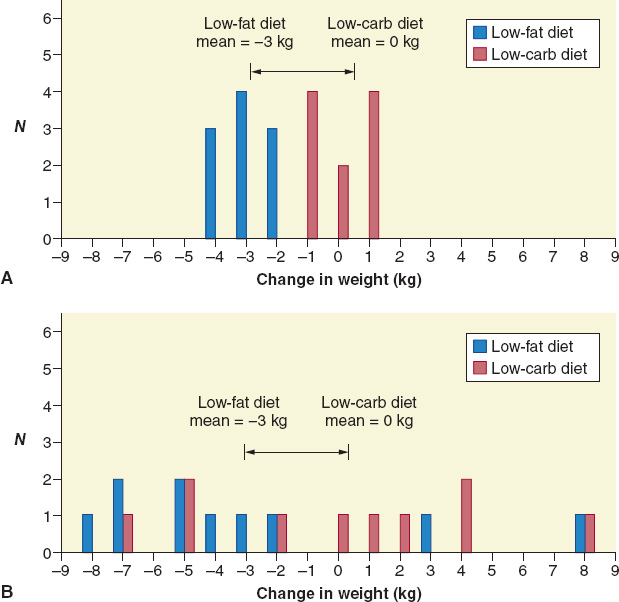
\includegraphics[width=15.3cm]{assets/ch05_diet_weight_loss.jpeg}};
\begin{scope}[x={(image.south east)},y={(image.north west)},font=\small]
\node[fill=chfivecream,inner sep=2pt,align=center,text width=2.55cm] at (.397,.945) {低脂饮食\\均值 $=-3$ kg};
\node[fill=chfivecream,inner sep=2pt,align=center,text width=2.55cm] at (.605,.945) {低碳水饮食\\均值 $=0$ kg};
\node[fill=chfivecream,inner sep=2pt,align=center,text width=2.55cm] at (.385,.313) {低脂饮食\\均值 $=-3$ kg};
\node[fill=chfivecream,inner sep=2pt,align=center,text width=2.55cm] at (.590,.313) {低碳水饮食\\均值 $=0$ kg};
\foreach \y in {.947,.426}{\node[fill=white,inner sep=1.5pt,align=left,text width=2.4cm,anchor=west] at (.789,\y) {低脂饮食};}
\foreach \y in {.909,.388}{\node[fill=white,inner sep=1.5pt,align=left,text width=2.4cm,anchor=west] at (.789,\y) {低碳水饮食};}
\foreach \y in {.535,.013}{\node[fill=white,inner sep=2pt,text width=6cm,align=center] at (.55,\y) {体重变化（kg）};}
\end{scope}
\end{tikzpicture}}

\sourcepage{102}
决定研究谁、研究什么以及采用何种设计后，研究者必须确定抽取多少参与者。也可能她已知道潜在人数，想判断是否足以使研究值得开展。样本过小，即使实施再周密，也可能无法为回答问题作出有意义的贡献；样本过大，又会使难度与费用超过必要程度，甚至检出小到没有临床意义的差异。样本量规划的目标，是针对给定设计估计适当人数。

即使人数已固定，例如参与者已经入组或数据已经收集，也值得了解样本量估算方法。稍后会看到，此时重要的是这个样本量能在多大程度上回答问题。

本书很早就介绍这一内容，是有原因的。经验表明，许多初学者花费大量精力设计，最后却因为所需样本量超过自身能力而无法实施。最好在设计初期就认清问题，以便还有时间修改，甚至重新考虑问题和计划。幸运的是，只要包含下文所说的明确研究假设，即使一页简单计划，通常也足以作出初步估算。
\sourcepage{103}
样本量计算虽然有用，却会给人一种具有统计客观性的错觉。它的准确程度，只能与依据的数据和估计一样，而这些估计往往只是有知识根据的猜测。最好把样本量规划看成用数学方法作粗略估算。它常会揭示设计不可行，或需要换用预测、结局变量。因此，应在仍可作重大调整的设计早期估计样本量。

第 6 章介绍几种常见设计的具体方法之前，我们先讨论原理。有些原理即使令人困惑，也不必完全掌握才能规划样本量；正如了解原料能使食谱更好理解，熟悉基本概念也能使计算更容易。即使打算请生物统计学家帮忙，理解过程，也能让你参与讨论计算中的假设和估计。

\section{假设}
首先，把研究问题改写为\term{研究假设}，概括样本、预测变量和结局变量等主要组成。例如，若问题是做填字游戏者是否较少发生痴呆，假设就须说明样本（如退休社区中认知正常者）、预测变量（平均每周至少做一次填字游戏）及结局变量（随访两年后标准认知测验评分异常）。

描述某特征在人群中分布的描述性研究，例如退休社区认知异常的患病率，本身不需要假设。
\sourcepage{104}
但这并不表示不必估算样本量，只是方法不同，见第 6 章。用显著性检验比较组间发现的分析性研究，例如上述填字游戏与痴呆问题，则需要假设。大多数观察性研究及所有实验都涉及比较，因此大多数研究至少需要一个假设。问题中若出现“大于”“小于”“更可能”“与……有关”“相比”“相关”“相似”“预测”“引起”“导致”等词，就不只是描述，应形成研究假设。

\subsection{好的研究假设具有什么特征}
好的假设必须以好的问题为基础，也应简单、具体并预先提出。
\subsubsection{简单与复杂}
\term{简单假设}（simple hypothesis）只包含一个预测变量和一个结局变量：
\begin{studyquote}在 II 型糖尿病患者中，久坐生活方式与发生蛋白尿的风险增加有关。\end{studyquote}
这里久坐生活方式是预测变量，发生蛋白尿是结局变量，两者都是二分类。

\term{复杂假设}（complex hypothesis）包含多个预测变量：
\begin{studyquote}在 II 型糖尿病患者中，久坐生活方式和饮酒与发生蛋白尿的风险增加有关。\end{studyquote}
或者包含多个结局变量：
\sourcepage{105}
\begin{studyquote}在 II 型糖尿病患者中，饮酒与发生蛋白尿和神经病变的风险增加有关。\end{studyquote}
这类复杂假设难以用单一统计检验处理，拆成两个或多个简单假设更容易。不过，有时可以合并预测或结局变量：
\begin{studyquote}在 II 型糖尿病患者中，饮酒与发生微血管并发症（蛋白尿、神经病变或视网膜病变）的风险增加有关。\end{studyquote}
最后这个例子中，研究者认为重要的是是否发生并发症，而不是哪一类并发症。

\subsubsection{具体与含糊}
具体假设不会让参与者、变量或显著性检验方法产生歧义。它用简明的操作性定义，概括参与者性质、来源及测量方法：
\begin{studyquote}在 Longview 医院因心肌梗死住院的患者中，既往使用三环类抗抑郁药至少六周，比因肺炎住院的对照更常见。\end{studyquote}
这句话虽长，却清楚传达了研究性质，尽量避免研究者看过结果后改检验略有不同的事项。比如，分析阶段若改用自报抑郁作为预测因素，却不考虑多重假设检验及数据操弄问题，就不正确；本章末将讨论这些问题。为保持简洁，某些细节通常在计划中说明，而不全写进假设。
\sourcepage{106}
从假设通常能看出预测及结局是二分类、连续还是其他分类变量。不清楚时，可以说明变量类型：
\begin{studyquote}在 35～59 岁非肥胖男性中，至少每周参加一次保龄球联赛，与十年随访中发生肥胖（BMI $>30$ kg/m$^2$）的风险增加有关。\end{studyquote}
同样，若假设过于冗长，可以把定义留到计划中澄清。

\subsubsection{预先与事后提出}
应在研究前，预先（a priori）用书面明确假设。这样可以把工作集中在主要目标，为解释结果提供更有力依据，并防止在数据里搜寻“阳性”结果。看过数据后形成的\term{事后假设}（post hoc hypotheses），属于多重假设检验，可能使人过度解释结果的重要性。把事后提出的假设冒充预先假设，是一种科研不端。

\subsection{零假设与备择假设}
提醒：如果从未正式学习统计，或已忘记所学，接下来几段第一次甚至前几次阅读时，可能难以理解。即使术语繁琐或令人困惑，也请努力读下去。

首先，把研究假设改写为“所比较组别之间没有差别”。这就是\term{零假设}（null hypothesis），它是研究结束后分析数据时，显著性检验的正式基础。假定零假设为真，也就是总体中确实不存在关联，
\sourcepage{107}
统计检验就能帮助估计研究中所见关联仅由偶然因素产生的概率。

例如，问题是饮用未净化井水是否与消化性溃疡风险增加有关，可能因为井水更易被幽门螺杆菌污染。研究采用病例对照设计，把溃疡病例与同一门诊中患下消化道疾病的对照比较。总体中预测与结局无关联的零假设，就是：
\begin{studyquote}消化性溃疡病例与对照饮用未净化井水的可能性相同。\end{studyquote}
认为存在关联，即“溃疡病例饮用未净化井水的可能性大于对照”，称为\term{备择假设}（alternative hypothesis）。它不能直接检验；如果显著性检验拒绝零假设，就默认接受备择假设，见后文。

\section{统计学基本原理}
研究假设，例如“每天运动至少 15 分钟与中年糖尿病女性较低的平均空腹血糖有关”，在现实中非真即假。研究者无法研究所有中年糖尿病女性，只能在目标人群样本中检验。如图 1.5 所述，始终需要从样本事件推断总体中的现象。\footnote{译注：底本此处写作图 1.5；所提供第五版第 1 章的图号为 1.1～1.4。此处保留原引用。}不幸的是，单凭偶然性，有时样本发生的事情并不反映研究整个总体时会发生的事情。

某种程度上，这类似陪审团判定被告是否有罪（表 5.1）。通常无法绝对确定被告是否犯罪，因此先推定无罪，再决定是否有足够依据，以“排除合理怀疑”为标准否定无罪推定。
\sourcepage{108}
但陪审团也会出错：把无辜者定罪，或未把有罪者定罪。
\begin{bookbox}{表 5.1\quad 陪审团裁决与统计检验的类比}
\begin{tabularx}{\linewidth}{YY}
\toprule 陪审团裁决 & 统计检验\\\midrule
无罪：被告未伪造货币。 & 零假设：中年糖尿病女性中，规律运动与平均空腹血糖无关联。\\
有罪：被告伪造了货币。 & 备择假设：规律运动与平均空腹血糖有关联。\\
否定无罪的标准：排除合理怀疑。 & 拒绝零假设的标准：显著性水平 alpha（$\alpha$）。\\
正确裁决：把伪造者定罪。 & 正确推断：总体确有运动与血糖关联时，得出存在关联的结论。\\
正确裁决：宣告无辜者无罪。 & 正确推断：总体无关联时，得出无关联的结论。\\
错误裁决：把无辜者定罪。 & 错误推断（I 类错误）：实际无关联，却得出存在关联的结论。\\
错误裁决：宣告伪造者无罪。 & 错误推断（II 类错误）：实际有关联，却得出无关联的结论。\\\bottomrule
\end{tabularx}
\end{bookbox}
\sourcepage{109}
同样，研究者先假定总体中预测与结局无关联，再根据样本资料，用统计检验判断是否有足够依据拒绝零假设、接受总体存在关联的备择假设。

\subsection{I 类与 II 类错误}
像陪审团一样，研究者也可能得出错误结论。有时只是偶然，样本不能代表总体，结果不反映总体实情，导致错误推断。总体中零假设实际为真，却被拒绝，是\term{I 类错误}（type I error，假阳性）；总体中零假设实际为假，却未被拒绝，是\term{II 类错误}（type II error，假阴性）。两类错误都无法完全避免，但增加样本量可降低概率，因为大样本不易与总体严重不同；调整设计或测量等方法也能降低概率，后文会讨论。

本章及下一章，只处理由偶然变异，即随机误差造成的 I 类和 II 类错误。偏倚也会产生假阳性或假阴性，但通常不称为 I 类或 II 类错误。偏倚造成的错误难以察觉，通常也不能用统计方法量化或靠扩大样本避免，因此很棘手。第 3、4、8～13 章介绍减少偏倚错误的方法。

\subsection{效应量}
研究能否在样本检出预测与结局的关联，取决于总体中关联的实际大小。关联大，例如空腹血糖差 20 mg/dL，较容易检出；
\sourcepage{110}
关联小，例如只差 2 mg/dL，就难以检出。

研究者几乎从不知道关联的准确大小，研究目的之一正是估计它。她必须选择希望在样本中检出的总体关联大小，这叫\term{效应量}（effect size）。选择适当效应量，也许是样本量规划最难的部分（1）。可以寻找相关领域既往资料，对合理效应量作有根据的猜测；或者选择自己认为具有临床意义的最小效应，例如空腹血糖降低 10 mg/dL。

当然，从公共卫生角度，即使降低 2～3 mg/dL 也可能重要，尤其容易实现时。效应量选择始终带有任意性，可行性常占首位。可用或负担得起的人数有限时，研究者可能需要反推（第 6 章）：在可研究人数下能检出多大效应，再判断是否合理。

许多研究测量不同预测及结局变量，因此有多个效应量。设计时应按最重要假设所需效应量确定样本量，再估计其他假设可检出的效应量。若多个假设同样重要，就采用所需样本量最大的那一个。

\subsection{Alpha、Beta 与效能}
研究结束后，研究者用统计检验拒绝零假设、接受备择假设，类似检察官说服陪审团否定无罪、判定有罪。假设研究无偏倚，视总体中零假设真假而定，
\sourcepage{111}
会有四种情形（表 5.2）。其中两种，样本发现与总体实际一致，推断正确；另两种则发生 I 类或 II 类错误，推断错误。
\begin{bookbox}{表 5.2\quad 总体实情与研究样本结果：四种可能}
\begin{tabularx}{\linewidth}{YYY}
\toprule & \multicolumn{2}{c}{总体中的实情}\\
样本中的结果 & 预测与结局有关联 & 预测与结局无关联\\\midrule
拒绝零假设 & 正确 & I 类错误\\
未拒绝零假设 & II 类错误 & 正确\\\bottomrule
\end{tabularx}
\end{bookbox}
研究前应确定对仅由偶然造成两类错误的容忍程度。偶然犯 I 类错误，即零假设真实却被拒绝，所允许的最大概率称\term{alpha}，也称\term{统计学显著性水平}（level of statistical significance）。

例如，以 $\alpha=0.05$ 设计规律运动与空腹血糖研究，就表示如果零假设为真，错误拒绝它的最大概率设为 5\%；即总体实际无关联时，错误推断有关联的概率。这是研究者在研究结束后进行统计检验时，愿意接受的“合理怀疑”程度。

犯 II 类错误，即零假设实际为假却未被拒绝的概率，称\term{beta}。$1-\beta$ 称\term{效能}（power），即总体真实效应等于指定效应量时，样本中正确拒绝零假设的概率。
\sourcepage{112}
设 $\beta=0.10$，就表示愿意接受漏掉真实存在的指定大小关联的概率为 10\%；等价于效能 0.90，即正确拒绝零假设的概率 90\%。例如，若总体糖尿病女性规律运动确实平均降低血糖 20 mg/dL，而研究者以相同的 90\% 效能反复开展研究，我们预期 90\% 的研究会在指定 alpha 下正确拒绝零假设，认为运动与空腹血糖有关联。这不表示她无法发现更小效应，例如降低 15 mg/dL，只是发现它的概率会低于 90\%。

理想情况下，alpha 与 beta 都应接近零，以尽量减少假阳性和假阴性。但降低它们，需要增加样本量或采取第 6 章介绍的其他办法。规划目标是在不使研究无谓昂贵或困难的条件下，选择足够人数，把两类概率保持在可接受的低水平。

许多研究设 $\alpha=0.05$、$\beta=0.20$，即效能 0.80。这些数值带有任意性；常用 alpha 范围 0.01～0.10，beta 范围 0.05～0.20。若特别需要避免 I 类假阳性，例如检验可能危险药物的疗效，就应设较低 alpha。若特别需要避免 II 类假阴性，例如向公众说明居住在有毒废物倾倒场附近安全，就应设较低 beta，并选择较小效应量。最后，如果研究容易、对参与者无风险或不便，例如资料早已收集，即使效能明显低于 0.80，也可能值得开展。

\subsection{备择假设的侧数}
\sourcepage{113}
备择假设可为单侧或双侧。\term{单侧备择假设}（one-sided alternative hypothesis）规定关联方向，例如饮井水增加溃疡风险。\term{双侧备择假设}（two-sided alternative hypothesis）只说有关联，不规定方向，例如“与饮用其他水相比，井水与不同的消化性溃疡风险有关，可能升高，也可能降低”。

只有一个方向具有临床或生物学意义的特殊情况下，才可能适合单侧假设。例如，新降压药比安慰剂更易引起皮疹，通常不值得检验它是否反而减少皮疹，除非药物有抗炎作用。在少数只关心一侧的情形，例如判断新抗生素是否不差于现行药物的非劣效性试验（第 12 章），可以据此计算样本量。但绝不应只为减少样本量而采用单侧假设。

研究假设通常是单侧，规划样本量所用的备择假设却几乎总是双侧，应注意两者区别。例如“儿童期反复使用抗生素，与炎症性肠病风险增加有关”，规定了预期方向，属于单侧。但大多数情况下，风险增加或降低都值得关注，无论哪个方向，研究者都希望发表，所以样本量仍应按双侧规划。必须在分析前选择单侧或双侧；事后为了减小 $P$ 值而从双侧改为单侧是不正确的。
\sourcepage{114}
此外，多数资助与稿件评审者期待双侧假设；没有充分理由时，他们会强烈质疑单侧做法，这或许才是双侧更常用的真正原因。

\subsection{\texorpdfstring{$P$}{P} 值及其局限}
现在可回到零假设。它只有一个作用，像一个“稻草人”：先假定它为真，再通过统计检验拒绝它。分析时，统计检验给出\term{$P$ 值}（P value）：如果零假设实际为真，仅由偶然产生与研究所见一样大或更大效应的概率。\footnote{为便于阅读，这里略去了统计细节。实际先计算在零假设下分布已知的检验统计量，例如 $t$ 统计量；$P$ 值是零假设为真时，获得至少同样极端统计量的概率。一项研究有时可用不止一种统计量，所以同一观察效应量可能有多个 $P$ 值。因此应预先指定检验，以免被认为在“$P$ 值操纵”（P-hacking），即尝试多种分析，寻找所希望的结果。}

关键在于：若零假设为真，总体两组确无差异，那么无偏倚研究在样本中发现差异，就只能归于偶然。（处理偏倚的方法见第 10 章。）

若 $P$ 值小于预定 alpha，就可以拒绝无差异的零假设，接受存在差异的备择假设。但不显著，即 $P$ 大于 alpha，并不表示总体无关联，而只说明样本所见关联可能仅由偶然产生。例如 $P=0.56$ 表示，若总体无关联，仅由偶然，超过一半时候会出现与研究所见大小相似的关联。

双侧检验的 $P$ 值包括两个方向，例如错误认为风险升高或降低，犯 I 类错误的概率，约为任一单独方向的两倍。因此，单侧 $P=0.05$ 通常等于双侧 $P=0.10$。
\sourcepage{115}
某些检验不对称，所以说“通常”。

例如，研究发现，参加大学校际运动的女性，以后接受全髋置换的可能性是未参加者的两倍，但也许人数有限，$P$ 值“仅”为 0.08。这表示即使总体中运动与髋置换无关联，偶然发现至少同样大的关联，仍有 8\% 概率。若原来采用双侧假设，设双侧 $\alpha=0.05$，就须判定“不具统计学显著性”。她可能想改报单侧 $P=0.04$，但更好的方法是报告结果及 95\% 置信区间，并说明“结果提示可能存在关联，但未达统计学显著性（$P=0.08$）”。这样既保留原来双侧设计，也承认统计学显著性并非非有即无。

确有一些流行病学家和统计学家反对设计时设置任意 $P$ 值界限（2、3）。但替代方法（4），例如估计研究信息的成本和价值，也依赖自己的假设；对于设计阶段，尤其是资助前须经同行评审的研究，目前还不十分实用。至少现在，本章及下一章的方法仍是临床研究的通用做法，也为更高级方法奠定基础。

尽管如此，绝不应仅报告“$P<0.05$，有统计学显著性”。更重要的是预测与结局关联有多大，以及估计有多精确，通常用置信区间表达（5）。

\sourcepage{116}
\subsection{统计检验的类型}
样本量公式依赖数学假定，而每种检验假定不同。计算前，必须决定数据分析方法；选择主要取决于预测及结局变量的类型。表 6.1 列出常用统计方法，第 6 章据此介绍简化估算方法。

\section{其他要点}
\subsection{变异性}
重要的不只是效应大小，还包括变异程度。统计检验需要显示组间差异；参与者结局变量的散布越大，两组越容易重叠，就越难显示总体差异。测量误差也是总变异的一部分，因此不精密测量需要更大样本（6）。

例如，40 人试验比较低脂与低碳水化合物饮食的减重效果。如果低脂组每人约减 3 kg，低碳水组几乎不减重，即效应量 3 kg，则低脂饮食很可能确实更好（图 5.1A）。但即使两组平均仍分别减 3 kg 和 0 kg，若两组大量重叠（图 5.1B），较大变异就使差异更难检出，需要更大样本。
\sourcepage{117}
\par
\begin{figure}[htbp]\centering\chfivediets
\caption*{\textbf{图 5.1}\quad \textbf{A：}两种饮食的减重效果。低脂组所有人减重 2～4 kg，低碳水组体重变化为 $-1$～$+1$ kg。两组不重叠，因此可合理认为低脂饮食减重更好；双样本配对 $t$ 检验也会证实，$P<0.001$。\textbf{B：}两组体重变化大量重叠。效应量虽然与 A 相同，均为 3 kg，却不足以认为一种饮食优于另一种；双样本配对 $t$ 检验 $P=0.19$。图中 $N$ 为人数。译注：底本两处均写作 two-sample paired t test，此处保留其“配对”措辞。}
\end{figure}\par
\sourcepage{118}
样本量估算中若有连续变量，例如图 5.1 体重变化，就需要估计其变异程度，具体见第 6 章 $t$ 检验部分。其他情形中，变异已由用于计算的其他参数包含，不必另行指定。

\subsection{多重假设与事后假设}
检验多个假设，至少一个仅凭偶然达到显著性的可能性就会上升。例如，以 $\alpha=0.05$ 检验 20 个独立假设，至少一个偶然显著的概率高达 $1-0.95^{20}=64\%$。一些统计学家主张，多假设时调整显著性水平，使所有结果都仅由偶然造成时，接受任何一个备择假设的总体概率仍保持在指定水平。例如，检验数千基因型与疾病关联的基因组研究，需要远低于 0.05 的 alpha，否则会发现大量假阳性关联。

一种方法以意大利数学家 Carlo Emilio Bonferroni 命名，称\term{Bonferroni 校正}（Bonferroni correction）：将显著性水平除以检验假设数。四个假设时，每个的 alpha 为 $0.05/4=0.0125$，而不是 0.05，这需要明显增加样本。因此，对任一假设，它以提高 II 类错误概率或增加样本量，换取 I 类错误概率下降。校正后仍显著，则效能损失不成问题；但若因此不显著，未能支持总体中真实存在的关联，即 II 类错误，就更麻烦。
\sourcepage{119}
尤其此时，使用何种显著性水平，更应取决于每个假设的\term{先验概率}（prior probability），而非假设数。因此，我们认为 Bonferroni 对多重假设通常过于严格。可借诊断检查作类比（7、8）：解释结果时，医师会考虑患者本来患病的可能性。例如，健康者的血清碱性磷酸酶仅高于正常上限 15\%，很可能是假阳性，临床意义有限。同样，一个本来不大可能成立的假设，即使 $P=0.05$，也很可能是假阳性。

但若碱性磷酸酶高出上限 10～20 倍，通常不易由偶然解释，虽然可能是实验室错误。同样，极小的 $P$ 值，如 $<0.001$，不大可能仅由偶然产生，虽然可能源于偏倚。即使疾病或假设先验概率低，也很难把极异常检查一概视为假阳性，或把极低 $P$ 值一概归于偶然。\footnote{例外是某些遗传学研究，可能检查数百万甚至数十亿个关联。}不过，即使 $P$ 极小，偏倚仍可解释，第 9 章会再讨论。

而且，检查或假设的数量并非总相关。患者关节肿痛、尿酸升高，如何解释不应取决于医师只查尿酸，还是在 20 项组合检查中获得该值。同样，解释一个有道理假设的 $P$ 值时，不应因研究者另外检验了几个不太可能的假设而改变。最重要的是假设本身合理，具有相当大的成立先验概率。在这种“贝叶斯”（Bayesian）思路中，先验概率常是基于其他来源资料的主观判断。设计阶段提出的假设通常满足这一条件；
\sourcepage{120}
否则，何必投入时间规划和研究？

那么，数据收集和分析中出现的意外关联呢？这有时叫“生成假设”，也有贬义的“数据挖掘”或“撒网捞鱼”。分析中的许多非正式比较，属于多重假设检验。分析时重新界定变量，或报告样本亚组结果，也有类似问题。设计阶段未考虑的事后假设，其显著 $P$ 值太常由偶然造成。应高度谨慎、清楚标明它由数据产生，最好把它当作未来研究问题的来源。任何情况下，都不得声称或暗示事后假设是在设计时构思的。

有时，研究者事先未明确某假设，但分析时看来合理。例如，研究过程中才发现一个新危险因素。这时重要的是，依据其他来源，是否有合理先验概率认为假设成立（7、8）。但仍须标明是事后假设。

为了分析中意外出现的不太可能结果编造解释，往往很诱人，却几乎没有统计学根据。正如物理学家 Richard Feynman 所说，事后几乎任何观察都可显得奇妙：“你知道，今晚发生了一件最神奇的事……我看见一辆牌照 ARW 357 的车。你能想象吗？全州几百万个车牌，今晚偏偏看到这一个，概率有多大？”（9）

不过，设计时提出多个假设也有优点。多个不相关假设可以提高效率，用一次研究回答更多问题，发现更多总体真实关联。
\sourcepage{121}
例如，研究红肉摄入等膳食预测因素与结直肠癌风险的队列，如果额外资料容易收集，也可以考察心血管结局。

提出几个相关假设也可能有益：结果一致会加强结论。例如，心力衰竭患者研究发现，血管紧张素转换酶抑制剂可减少心脏相关住院、心血管死亡和总死亡。若只检验其中一项，推断就不那么确定。然而，检验几个相关或改写的假设又有问题：如果只有一个显著，其他远不显著，研究者就必须判断并说服编辑和读者，究竟是显著结果、不显著结果，还是两者都正确。

\subsection{主要假设与次要假设}
有些研究，尤其大型随机试验，会指定次要假设。通常研究围绕一个主要假设设计，但研究者也对较次要问题感兴趣。例如，补锌试验的主要结局可能是因上呼吸道感染就医，次要结局可能是自报缺勤或缺课天数。若为药物审批开展研究，监管方最重视主要结局。预先提出少数次要假设，可以增加其结果可信度；但次要假设越多，每个的可信度越低。
\sourcepage{122}
一个好规则，尤其适用于临床试验，是事先提出合理数量的假设，但只指定一个主要假设，这样检验它时就不必争论是否需多重校正。更重要的是，主要假设能使研究聚焦主要目标，并为主要样本量计算提供清楚依据。

\section{小结}
\begin{enumerate}
\item 样本量规划对分析性及描述性研究都很重要；应在制订计划早期估算，以便调整。
\item 分析性研究和实验，需要针对后续统计检验，明确主要预测与结局的预期关联假设。纯描述性研究没有比较，不需要假设。
\item 好的假设具体说明抽样人群和测量变量，简单到只有一个预测和一个结局，并事先提出。
\item 零假设认为预测与结局无关联，是显著性检验基础；备择假设认为有关联。统计检验尝试拒绝前者、接受后者。
\item 备择假设可单侧或双侧。只有一个方向有临床或生物学意义的特殊情形，才应使用单侧。
\item 分析性研究与实验的样本量，是在给定效应量及变异程度，以及指定 I 类、II 类错误概率下，检出关联所需的人数估计。
\sourcepage{123}
I 类错误的最大概率叫 alpha，II 类叫 beta；$1-\beta$ 是效能，即总体确有给定效应时，在样本中观察到关联的机会。
\item 事先提出不止一个假设通常有益，但应指定一个主要假设，作为研究及样本量估计的中心。解释多个假设的结果，包括数据中出现的意外发现，要判断其代表总体真实现象的先验概率。
\end{enumerate}
\begin{references}
\item Van Walraven C, Mahon JL, Moher D, et al. Surveying physicians to determine the minimal important difference: implications for sample-size calculation. J Clin Epidemiol. 1999;52:717-723.
\item Goodman SN. Toward evidence-based medical statistics. 1: the P value fallacy. Ann Intern Med. 1999;130:995-1004.
\item Goodman SN. Toward evidence-based medical statistics. 2: the Bayes factor. Ann Intern Med. 1999;130:1005-1013.
\item Bacchetti P. Current sample size conventions: flaws, harms, and alternatives. BMC Med. 2010;8:17.
\item Daly LE. Confidence limits made easy: interval estimation using a substitution method. Am J Epidemiol. 1998;147:783-790.
\item McKeown-Eyssen GE, Tibshirani R. Implications of measurement error in exposure for the sample sizes of case-control studies. Am J Epidemiol. 1994;139:415-421.
\item Browner WS, Newman TB. Are all significant P values created equal? The analogy between diagnostic tests and clinical research. JAMA. 1987;257:2459-2463.
\item Newman TB, Kohn MA. Evidence-Based Diagnosis: an Introduction to Clinical Epidemiology. 2nd ed. Cambridge University Press; 2020:285-289.
\item Feynman R, Leighton R, Sands M. Six Easy Pieces: Essentials of Physics Explained by Its Most Brilliant Teacher. Basic Books; 2011.
\end{references}
\sourcepage{124}
\chapterappendix{5A}{第 5 章习题：样本量估计的准备}
\sourcepage{125}
\begin{enumerate}
\item 定义下列文字中用红色标示的概念。

研究者准备设计一项\term{样本量}充足的研究，确定 50～75 岁女性的 BMI 是否与胃癌有关。她计划病例与对照人数相等的病例对照研究。\term{零假设}是两组平均 BMI 无差别；选择的\term{备择假设}为双侧。她希望在\term{统计学显著性水平（alpha）}0.05 下，具有 0.80 的\term{效能}，检出病例与对照 BMI 相差 1 kg/m$^2$ 的\term{效应量}。文献显示，女性 BMI 的\term{变异性}可用标准差 2.5 kg/m$^2$ 表示。
\item 以下哪项可能是 I 类错误，哪项可能是 II 类错误，哪项两者都不是？
\begin{enumerate}
\item 随机试验发现，新镇痛药组的平均疼痛评分降幅大于安慰剂组（$P=0.03$）。
\item 十年研究报告，110 名吸烟者的肺癌发病率未高于 294 名不吸烟者（$P=0.31$）。
\item 研究者写道：“本研究首次发现，饮酒降低 50 岁以下男性的糖尿病风险（$P<0.05$）。”
\end{enumerate}
\end{enumerate}
